\chapter{Definição do Problema de Estudo}

A estrutura básica de um veículo elétrico é exibida na Figura
\ref{fig:estrutura-veiculo-eletrico}. O bloco conversor CA-CC no diagrama representa todo o
carregador \textit{onboard} do veículo elétrico, incluindo tanto o retificador PFC quanto o
conversor CC-CC isolado. O sistema de carregamento pode ser unidireccional ou bidirecional. No
primeiro caso, o sistema apenas converte a energia da rede elétrica para o veículo, enquanto no
segundo caso, o veículo pode fornecer energia de volta para a rede elétrica, o que é conhecido
como \textit{Vehicle-to-Grid} (V2G). O banco de baterias do veículo é composto por células de
lítio e ultracapacitores, que são ulizados para armazenar a energia elétrica fornecida pelo
carregador. O inversor é responsável por converter a tensão CC da bateria em uma tensão CA, que
aciona o motor do sistema de tração do veículo. Como ilustrado no diagrama, o inversor
geralmente é bidirecional, o que permite o uso de frenagem regenerativa.

Os carregadores de veículos elétricos são divididos em carregadores \textit{onboard}(OBC) e
\textit{offboard}. Os carregadores \textit{onboard} são instalados dentro do veículo e são
projetados para serem leves e compactos, devido a restrições de espaço e peso. A potência de
saída desses carregadores está na faixa de 0 a 7 kW para sistemas monofásicos e de 0 a 22 kW
para sistemas trifásicos \cite{Yuan:2021}. Já os carregadores \textit{offboard} também são
chamados de carregadores nível 3 e já fornecem uma tensão CC direta para o veículo, ignorando o
OBC conforme ilustrado em \ref{fig:estrutura-veiculo-eletrico}. A potência de saída desses
carregadores é significativamente maior, variando de 120 kW a 240 kW, segundo
\cite{texas:2020}.

\begin{figure}[htb]
    \centering
    \caption{Estrutura básica de um veículo elétrico.}
    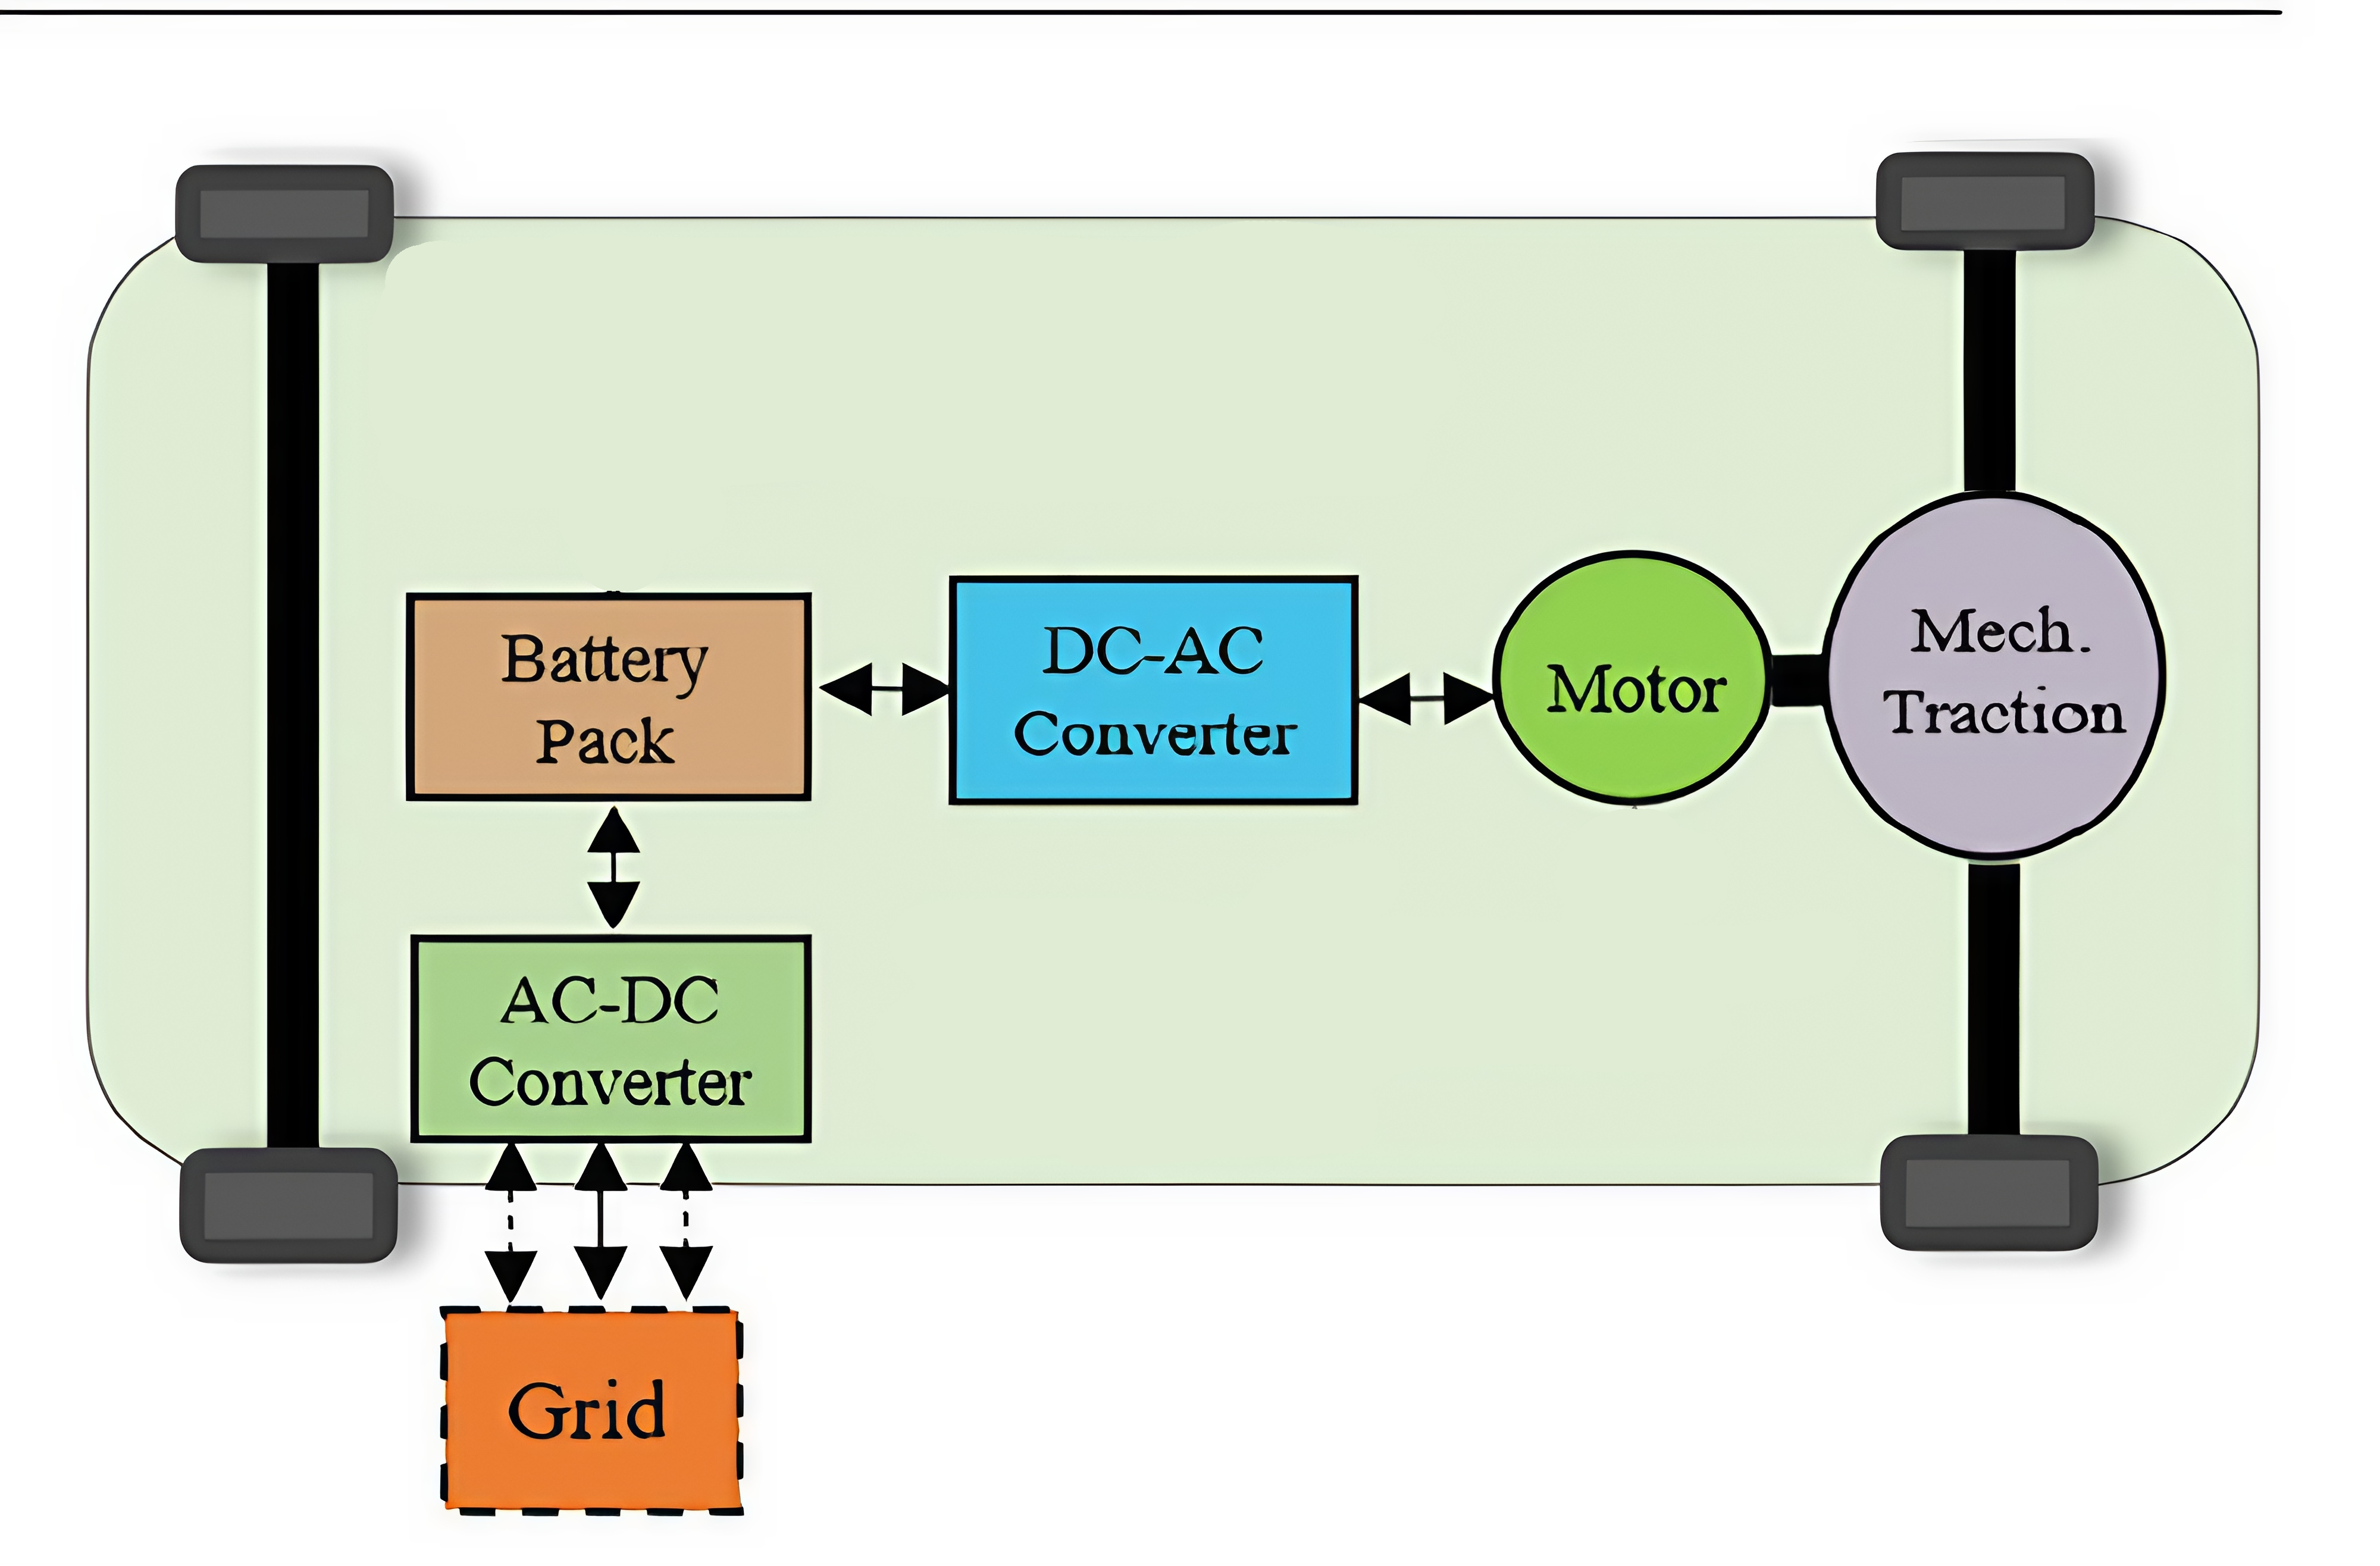
\includegraphics[width=0.8\textwidth]{figuras/diagrama_veiculo_eletrico_edit.png}
    \legend{Fonte: Adaptado de \cite{Kumar:2021}.}
    \label{fig:estrutura-veiculo-eletrico}
\end{figure}

\begin{figure}[htb]
    \centering
    \caption{Sistema de carregamento \textit{offboard}. Há uma conexão direta entre o
        carregador e a bateria do veículo.}
    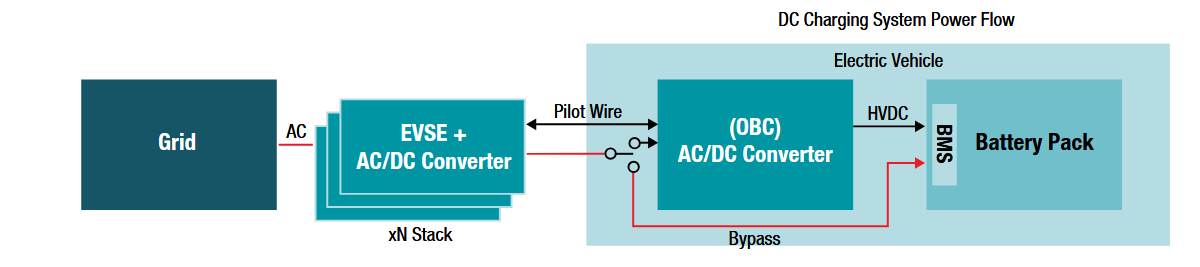
\includegraphics[width=0.8\textwidth]{figuras/diagrama_bypass.png}
    \legend{Fonte: \cite{texas:2020}.}
    \label{fig:diagrama-bypass-offboard}

\end{figure}

A crescente demanda por veículos elétricos é impulsionada pela necessidade de reduzir emissões
de gases do efeito estufa e a dependência de combustíveis fósseis. De acordo com
\cite{anfavea2024descarbonizacao}, num cenário de transição gradual, é previsto que 65\% da
frota de veículos no Brasil seja elétrica até 2035. No entanto, a adoção em massa de veículos
elétricos enfrenta gargalos significativos, especialmente no que diz respeito à falta de
infraestrutura de carregamento e à baixa autonomia dos veículos elétricos \cite{Karneddi:2021}.

Ademais, os carregadores de veículos elétricos devem ser projetados para não afetar de forma
significativa a rede de distribuição elétrica, principalmente em relação ao fator de potência e
a distorção harmônica total. Nesse quesito, a normas técnicas IEC 61000-3 e GB/T 14549,
vigentes na União Europeia e na China, respectivamente, estabelecem limites de distorção
harmônica total e fator de potência para equipamentos conectados à rede elétrica. No Brasil, a
seção VIII da resolução 1000/2021 da ANEEL estabelece o fator de potência mínimo de 0,92 para
consumidores do grupo A, com cobrança de multa para excesso de energia reativa
\cite{aneel_ren1000_2021}.

Considerando os desafios encontrados para a crescente demanda em veículos elétricos, o seguinte
trabalho propõe o projeto de um carregador \textit{onboard} que seja adequado à realidade do
sistema de distribuição brasileiro. Dessa forma, escolhe-se trabalhar com um sistema de
carregamento trifásico que funcione com a rede de distribuição elétrica das grandes capitais
brasileiras, caracrterizada por uma tensão de fase de 127 \(V_{\mathrm{rms}}\) e uma frequência
de 60 Hz. O carregador será composto por um retificador PFC trifásico, que garante o fator de
potência próximo a unidade, e um conversor CC-CC isolado, que pode ser um \textit{Phase-Shifted
    Full Bridge}, um \textit{Dual Active Bridge}(DAB) ou um conversor ressonante. No trabalho será
realizado a comparação entre o \textit{Phase-Shifted Full Bridge} e o DAB com o objetivo de
verificar qual topologia apresenta melhor desempenho.

\section{Objetivo Geral}
O objetivo geral do trabalho é projetar um carregador de veículo elétrico \textit{onboard}
trifásico, composto por um retificador PFC e um conversor CC-CC isolado.
\section{Objetivos Específicos}
\begin{itemize}
    \item Realizar revisão bibliográfica sobre as diferentes topologias utilizadas no carregamento de
          carros elétricos;
    \item Projeto do circuito retificador PFC trifásico;
    \item Sintonia do controlador do retificador PFC trifásico;
    \item Projeto do conversor CC-CC \textit{Phase-Shifted Full Bridge};
    \item Projeto do conversor CC-CC \textit{Dual Active Bridge}(DAB);
    \item Comparação entre o \textit{Phase-Shifted Full Bridge} e o DAB.
\end{itemize}